% --- Template for thesis / report with tktltiki2 class ---
% 
% last updated 2013/02/15 for tkltiki2 v1.02

\documentclass[finnish]{tktltiki2}

% tktltiki2 automatically loads babel, so you can simply
% give the language parameter (e.g. finnish, swedish, english, british) as
% a parameter for the class: \documentclass[finnish]{tktltiki2}.
% The information on title and abstract is generated automatically depending on
% the language, see below if you need to change any of these manually.
% 
% Class options:
% - grading                 -- Print labels for grading information on the front
%page.
% - disablelastpagecounter  -- Disables the automatic generation of page number
%information
%                              in the abstract. See also
%\numberofpagesinformation{} command below.
%
% The class also respects the following options of article class:
%   10pt, 11pt, 12pt, final, draft, oneside, twoside,
%   openright, openany, onecolumn, twocolumn, leqno, fleqn
%
% The default font size is 11pt. The paper size used is A4, other sizes are not
%supported.
%
% rubber: module pdftex

% --- General packages ---

\usepackage[utf8]{inputenc}
\usepackage[T1]{fontenc}
\usepackage{lmodern}
\usepackage{microtype}
\usepackage{amsfonts,amsmath,amssymb,amsthm,booktabs,color,enumitem,graphicx}
\usepackage[pdftex,hidelinks]{hyperref}

% Automatically set the PDF metadata fields
\makeatletter
\AtBeginDocument{\hypersetup{pdftitle = {\@title}, pdfauthor = {\@author}}}
\makeatother

% --- Language-related settings ---
%
% these should be modified according to your language

% babelbib for non-english bibliography using bibtex
\usepackage[fixlanguage]{babelbib}
\selectbiblanguage{finnish}

% add bibliography to the table of contents
\usepackage[nottoc]{tocbibind}
% tocbibind renames the bibliography, use the following to change it back
\settocbibname{Lähteet}

% --- Theorem environment definitions ---

\newtheorem{lau}{Lause}
\newtheorem{lem}[lau]{Lemma}
\newtheorem{kor}[lau]{Korollaari}

\theoremstyle{definition}
\newtheorem{maar}[lau]{Määritelmä}
\newtheorem{ong}{Ongelma}
\newtheorem{alg}[lau]{Algoritmi}
\newtheorem{esim}[lau]{Esimerkki}

\theoremstyle{remark}
\newtheorem*{huom}{Huomautus}


% --- tktltiki2 options ---
%
% The following commands define the information used to generate title and
% abstract pages. The following entries should be always specified:

\title{OWL - Web Ontology Language}
\author{Hansi Keijonen}
\date{\today}
\level{Seminaariraportti}
\abstract{Tiivistelmä.}

% The following can be used to specify keywords and classification of the paper:

\keywords{avainsana 1, avainsana 2, avainsana 3}
\classification{} % classification according to ACM Computing Classification
%System (http://www.acm.org/about/class/)
                  % This is probably mostly relevant for computer scientists

% If the automatic page number counting is not working as desired in your case,
% uncomment the following to manually set the number of pages displayed in the
%abstract page:
%
% \numberofpagesinformation{16 sivua + 10 sivua liitteissä}
%
% If you are not a computer scientist, you will want to uncomment the following
%by hand and specify
% your department, faculty and subject by hand:
%
% \faculty{Matemaattis-luonnontieteellinen}
% \department{Tietojenkäsittelytieteen laitos}
% \subject{Tietojenkäsittelytiede}
%
% If you are not from the University of Helsinki, then you will most likely want
%to set these also:
%
% \university{Helsingin Yliopisto}
% \universitylong{HELSINGIN YLIOPISTO --- HELSINGFORS UNIVERSITET --- UNIVERSITY
%OF HELSINKI} % displayed on the top of the abstract page
% \city{Helsinki}
%


\begin{document}

% --- Front matter ---

\maketitle        % title page
\makeabstract     % abstract page

\tableofcontents  % table of contents
\newpage          % clear page after the table of contents


% --- Main matter ---
use case

\section{Johdanto}
Semanttinen web on visio tulevaisuuden webistä, jossa informaatiolle annetaan eksplisiittinen
merkitys mahdollistaen näin koneiden kyky prosessoida ja yhdistellä webissä olevaa tietoa \cite{MH04}.  
Tim Berners-Lee, James Hendler ja Ora Lassila toteavat
artikkelissa "Semantic web", että  
\begin{quote}
"Semanttinen web ei ole erillinen web vaan
laajennos tämänhetkiseen webiin, jossa informaatiolle on annettu hyvin muotoiltu
merkitys mahdollistaen koneiden ja ihmisten paremman yhteistyön. TULEEX VIITE MIHIN?"
\end{quote}
Suurin osa tämän päivän webin sisällöstä on tarkoitettu ihmisten luettavaksi sekä tulkittavaksi.
Kone pystyy tulkitsemaan esim. html-tiedoston ja esittämään
dokumentin siinä määritellyllä tavalla mutta se ei
\textit{ymmärrä} dokumentin sisällön merkitystä, semantiikkaa \cite{BHL01}.Tämä 
rajoittaa esimerkiksi haut internetissä olevista dokumenteista yksinkertaiseksi hakusanojen
etsimiseksi. Sen sijaan jos hakukoneet ymmärtäisivät asioiden merkityksen ja
niiden välillä vallitsevat yhteydet, olisivat hakutulokset tarkempia
ja sisältäisivät mahdollisesti laajennettuja hakuja alkuperäisen asian ympäriltä
\cite{SHIQ}. Semanttisella webillä on mahdollisuuksia myös verkkokaupankäynnissä, jossa 
myyjäagentit ja ostaja-agentit voivat kommunikoida keskenään tuotetietojen pohjalta luotujen 
ontologioiden avulla \cite{SHIQ}. Myös eri toimijoiden tuottamien web-palveluiden koostamisessa semanttisen 
webin teknologioilla on keskeinen rooli: palveluiden tuottajat voivat kuvata tarjoamansa
palvelun jolloin palveluita kokoavat sovellukset voivat niitä hyödyntää tehokkaasti \cite{SHIQ}. 
Maailmanlaajuinen tietoverkko tulisi siis muuttaa dokumenttien verkosta 
tiedon verkoksi \cite{BHL01}. 

Semantiikkaa voidaan webissä ilmaista ontologioilla. Tietojenkäsittelytieteessä
ontologialla tarkoitetaan dokumenttia, jossa kerrrotaan asioiden välisistä
yhteyksistä \cite{BHL01}.
Ontologioiden luomiseksi pitää olla menetelmiä käsitteiden määritykseen, käsitteiden
ominaisuuksien määritykseen sekä käsitteiden välisten suhteiden määritykseen
\cite{BHL01}. World Wide Web Consortium W3C on määritellyt 
joukon standardeja (suosituksia) kielille ja sanastoille, joilla merkitysten määrittäminen voidaan toteuttaa.
Tässä artikkelissa selvitetään pääasiassa OWL:n periaatteita. Lyhenne OWL tulee sanoista Web Ontology Language ja sille on
W3C:n suositus standardiksi vuodelta 2004. Uudempi suositus on OWL2:lle vuodelta 2012. 

Jotta olisi mahdollista ymmärtää OWL:n toimintaperiaate on käytävä soveltuvin osin läpi myös teknologiat, joihin
se perustuu. Tässä artikkelissa esitellään RDF ja RDF Schema, joiden konstruktioihin OWL vahvasti nojaa. 
Lopuksi selvitetään lyhyesti OWL:n laajennoksen OWL2:n tuomat lisäominaisuudet.  

\section{Teknologiat ja kielet jotka mahdollistavat OWL:n}
W3C tarjoaa semanttisen webin toteuttamiseen suositukset teknologioista ja
kielistä. Kuvassa \ref{stack} on semanttisen webin teknologia- ja konseptipino.
Osa teknologioista on jo todellisuutta ja
käytössä, osa vasta ideatasolla. Jokainen kerros hyödyntää alemman kerroksen toteuttamia
palveluita. Seuraavissa kappaleissa käydään läpi kaavion teknologioita ja kieliä
alhaalta ylöspäin kohti OWL:ää. Jokaisesta teknologiasta ja kielestä käsitellään tarkemmin
ne konstruktiot, jotka ovat olennaisia ja käytössä myös OWL:ssä.

\begin{figure}[h]
 \centering
 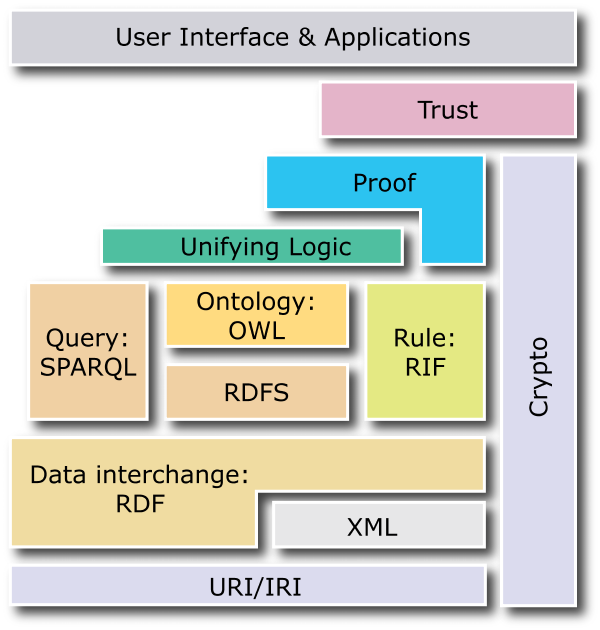
\includegraphics[scale=0.50]{stack.png}
 \caption{Semanttisen webin toteutukseen tarvittavat teknologiat, kielet ja konseptit. Lähde: http://commons.wikimedia.org/wiki/File:Semantic\_Web\_Stack.png }
 \label{stack}
\end{figure}
 
\subsection{URI ja XML}

Semanttisessa webissä määritettyjä luokkia, ilmentymiä, ominaisuuksia ja ominaisuuksien
arvoja kutsutaan resursseiksi \cite{BHL01}. Jotta sekaannusta jo määritettyjen resurssien
sekä uusien määritysten kanssa ei syntyisi, identifioidaan kaikki resurssit
yksilöllisesti URI(Unified Resource Identifier):n avulla.
URI:n avulla voidaan viitata mihin tahansa resurssiin webissä. Useimmiten
URIna toimii perinteinen URL(Unified Resourse Locator)-osoite \cite{BHL01}. IRI
(Internationalized Resource Identifier) on ainoastaan merkistölaajennos URI:in.
 
 Semanttisen webin kuvaukset toteutetaan useimmiten XML-kielellä.
XML-kieli on notaatio monimutkaisen rakenteisen tiedon esittämiseen ja
tarjoaa näin standardoidun mallin tiedon vaihtamiseen prosessoijien välillä.
Tärkeä XML:n ominaisuus on nimiavaruudet, jotka mahdollistavat ja helpottavat resurssien
identifiointia URI:en avulla. Nimiavaruuksien käyttöä selvitetään tarkemmin
OWL-ontologioiden yhteydessä. 

\subsection{Tiedon esittäminen RDF-triploilla}

Resource Description Framework RDF on kieli webissä olevien resurssien
kuvaamiseen \cite{RDFP}. 
RDF perustuu resurssien identifiointiin URI:lla ja näiden kuvaamiseen 
ominaisuuksilla ja ominaisuuksien arvoilla. Tämä mahdollistaa yksinkertaisten
lausumien esittämisen verkkoina, joissa resurssit ja ominaisuuksien arvot ovat soluja ja
ominaisuudet verkon 
kaaria \cite{RDFP}. % Kuvassa \ref{jack} on havainnollistettu asiaa. 

\begin{figure}[h]
 \centering
 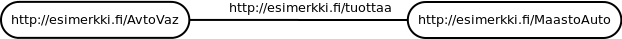
\includegraphics[scale=0.50]{JackTorrance.png}
 \caption{RDF-tripla joka kuvaa yksinkertaisen lausuman. Jokainen triplan solmu
ja kaari on identifioitu URI:lla. }
 \label{jack}
\end{figure}

Kuvassa \ref{jack} on kuvattu yksinkertainen \textit{RDF-tripla}.
Triplan subjekti, predikaatti ja objekti kertovat, että "Jack Torrance on ammatiltaan
kirjailija". Subjekti on siis asia, jota kuvataan, predikaatti on ominaisuus, jolla 
kuvataan ja objekti on ominaisuuden arvo \cite{RDFP}. 
Jokainen solu ja kaari on esimerkissä identifioitu URI:lla. Objekti voi olla
myös literaali, jolloin 
sitä ei identifioida erikseen, mutta formaatti voidaan määritellään esimerkiksi XML Scheman
datatyyppien avulla. 

Yleisin tapa esittää tripla on XML-notaatio. Myös muut tavat ovat mahdollisia,
kuten 
esimerkiksi \textit{JSON} \footnote{JSON on nönnöö} ja \textit{turtle} \footnote{turtle on nönnöö}. Alla on esitetty kuvassa
\ref{jack} esitetyn triplan XML-notaatio:
\begin{verbatim}
<?xml version="1.0"?>

<rdf:RDF
    xmlns:rdf="http://www.w3.org/1999/02/22-rdf-syntax-ns#"
    xmlns:ex="http://www.esimerkki.com/">
    
    <rdf:Description rdf:about="http://esim.fi/JackTorrance">
        <ex:onAmmatiltaan rdf:resource="http://esim.fi/Kirjailija"/>
    </rdf:Description>
</rdf:RDF>
\end{verbatim}
Esimerkistä näkee, kuinka subjekti (Jack Torrance)ja objekti (Kirjailija) ovat
identifioitu eksplisiittisellä URI:lla. Predikaattiin (onAmmatiltaan) viitataan myös URI:lla, mutta
nimiavaruuden kautta. Esimerkistä ilmenee RDF:n kolme peruskonstruktiota:  
\textit{rdf:Description} ilmoittaa, että kyseessä on kuvaus, \textit{rdf:about} viittaa subjektiin, \textit{rdf:resource}
viittaa resurssiin, tässä tapauksessa ominaisuuden arvoon. 

****tää seuraava on ihan kiva läppä, mutta onko paikka tässä? mahdollisesti ennen xml-esimerkkiä?***********
Jack Torrance on toiselta ammatiltaan talonmies ja myös Laila Hietamies
on ammatiltaan kirjailija. Kun myös nämä triplat lisätään kuvan \ref{jack} kaavioon, alkaa
pieni mutta informatiivinen verkko syntyä (kuva \ref{jack2}). Tästä verkosta voisimme
tehdä jo hakuja, kuten "listaa henkilöt, jotka ovat kirjailijoita".

\begin{figure}[h]
 \centering
 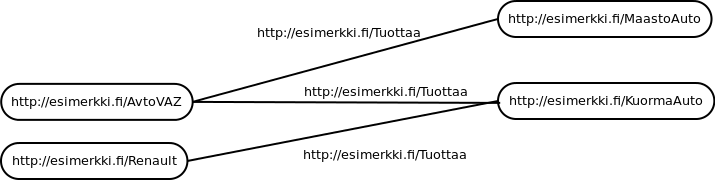
\includegraphics[scale=0.50]{torrance2.png}
 \caption{RDF-triplat muodostavat verkon.}
 \label{jack2}
\end{figure}

RDF tarjoaa melko alkeellisen tavan esittää lausumia, jotka
muodostavat haut mahdollistavan verkon. RDF toteuttaa myös joukon muita ominaisuuksia, kuten
\textit{säiliöitä} (container) tiedon säilömiseen sekä
\textit{kokoomatietorakenteita}
(collections) asioiden listaamiseen \cite{RDFP}. Näitä käsitellään myöhemmin
niiltä osin 
kuin ne ovat relevantteja OWL-ontologioiden muodostamisessa.  
 
\subsection{Yksinkertaiset ontologiat RDF Schemalla}

%RDF:llä ilmaistut ominaisuudet voidaan ajatella resurssien attribuuteiksi
%samassa mielessä kuin perinteiset attribuutti-arvo -parit \cite{RDFS}. 
Vaikka RDF:llä voidaan kuvata resursseja ominaisuuksien avulla ja määrittää näin resurssien välisiä suhteita, se ei tarjoa keinoja määrittää itse ominaisuuksia tai
ominaisuuksien välisiä suhteita \cite{RDFS}. Tämän mahdollistaa RDF:n \textit{sanastonkuvauslaajennos}
RDF Schema. RDF Schemalla on mahdollista määrittää resurssien joukkoja luokiksi (class) sekä näiden (luokkien ja yksilöiden) välisiä suhteita ominaisuuksiksi (property) \cite{RDFS}. 
RDF Schema on RDF:n semanttinen laajennos joka ei kuitenkaan tarjoa sanastoa asioiden ymmärtämiseen, vaan se tarjoaa työkaluja sanastojen luomiseen \cite{RDFS}. 

RDF Scheman yksi peruselementti on siis \textit{luokka}, jolla voi olla myös \textit{aliluokkia}. Luokan jäsenet ovat \textit{yksilöitä}, luokan \textit{ilmentymiä}. Toinen peruselementti on \textit{ominaisuus}. Ominaisuus yhdistää luokan 
ilmentymiä toisiinsa, luo suhteen niiden välille. Ominaisuudella voi olla myös \textit{aliominaisuuksia}. Näiden elementtien avulla voidaan määrittää melko yksinkertaisia luokkien ja suhteiden hierarkkisten järjestelmien kuvauksia, (kevyt)ontologioita.  

Seuraavissa kappaleissa esitellään niitä RDF Scheman peruskonstruktioita, 
joita myös OWL käyttää toteutuksessaan lähes sellaisenaan. \emph{RDFS Schema määrittelee myös suurehkon joukon muita konstruktioita, mutta niiden käsittely on OWL:n esittelyn kannalta tässä tarpeetonta.} 
Huomionarvoista on, että RDF Schema -dokumentit ovat RDF-dokumentteja, jotka sisältävät kummankin kielen primitiivejä. \textbf{Kaikissa tämän paperin koodiesimerkeissä on esitetty ainoastaan esittelyssä oleva konstruktio. Nimiavaruusmäärittelyt, otsikkotiedot jne. puuttuvat esimerkeistä yksinkertaisuuden vuoksi.}   

\subsubsection{Luokka ja yksilö}
Resurssit voidaan jaotella luokkiin. Luokkien jäseniä nimitetään luokan ilmentymiksi tai yksilöiksi\cite{RDFS}. Luokat ovat myös itse resursseja. Useimmiten luokat identifioidaan RDF:n URI:lla ja niitä voidaan kuvata RDF:n ominaisuuksilla (property). Luokka määritellään rdfs:Class elementissä. rdf:type -elementillä ilmaistaan, että resurssi kuuluu määrättyyn luokkaan \cite{RDFS}. Esimerkiksi kustannusosakeyhtiö "WSOY" on luokan "Kustantamo" jäsen:
\begin{verbatim}
    <rdfs:Class rdf:ID="WSOY" />
        <rdf:type rdf:resource="#Kustantamo"/>
    </rdfs:Class>
\end{verbatim} 

\subsubsection{Aliluokka}
rdfs:subClassOf -elementillä voidaan ilmaista, että kaikki jonkin luokan jäsenet ovat myös jonkin toisen luokan jäseniä \cite{RDFS}. Esimerkiksi 
luokka "Kustantamo" on luokan "Liikeyritys" aliluokka:
\begin{verbatim}
    <rdfs:Class rdf:ID="Kustantamo" />
        <rdf:subClassOf rdf:resource="#Liikeyritys"/>
    </rdfs:Class>
\end{verbatim}
Kaikki yksilöt, jotka kuuluvat luokkaan Kustantamo kuuluvat myös luokkaan Liikeyritys.
\subsubsection{Ominaisuus ja periytetty aliominaisuus}
Resursien välisiä suhteita kuvataan \textit{ominaisuuksilla}. Esimerkiksi "Matilla on veli Teppo". Voidaan ajatella, että resurssien "Matti" ja "Teppo" välinen suhde on ominaisuus "Veljeys". Ominaisuus "Veljeys" voi olla ominaisuuden "Perhesuhde"  aliluokka tai paremminkin aliominaisuus. Tällaisia konstruktioita kuvataan RDF Schemassa termillä subPropertyOf: 
\begin{verbatim}
    <rdf:Property rdf:about="Veljeys">
        <rdfs:subPropertyOf rdf:resource="#Perhesuhde" />
    </rdf:Property>

    <rdf:Description rdf:about="#Matti">
        <Veljeys rdf:resource="#Teppo" />
    </rdf:Description>
\end{verbatim}
Esimerkissä on määritetty ensiksi ominaisuus "Veljeys", joka on ominaisuden "Perhesuhde" aliominaisuus. Seuraavaksi kuvataan yksilöä "Matti" ominaisuudella "Veljeys", joka saa arvokseen resurssin "Teppo". subPropertyOf ilmaisee määritelmällisesti, että resurssit joiden välistä suhdetta kuvataan jollain suhteella, voidaan kuvata myös tämän suhteen ylisuhteella, josta ko. suhde on periytynyt \cite{RDFS}. Matin ja Tepon suhdetta voidaan kuvailla ominaisuudella "Veljeys", mutta myös ominaisuudella "Perhesuhde". 

\subsubsection{Rajoitukset ominaisuuden sovellusalueessa ja arvojoukossa}
RDF Schemassa on mahdollista määrittää ominaisuuksille rajoituksia sen suhteen, että minkä luokkien jäsenten välistä suhdetta ominaisuus voi kuvata. Ensinnäkin
voidaan rajoittaa ominaisuuden sovellusaluetta (domain). Esimerkiksi ominaisuuden "Työskentelee" sovellusalue voidaan rajata koskemaan ainoastaan luokkaa "Työntekijä". Samoin 
ominaisuuden saamat arvot (range) voidaan rajata olemaan ainoastaan luokan "Yritys" tai sen aliluokkien ilmentymiä: 
\begin{verbatim}
    <rdf:Property rdf:about="Tyoskentelee">
        <rdfs:domain rdf:resource="#Tyontekija" />
        <rdfs:range rdf:resource="#Yritys" />
    </rdf:Property>
\end{verbatim}
Sovellusalueen rajaus määritetään rdfs:domain -elementillä ja arvojoukon rajaus rdfs:range -elementillä.  

\section{Kehittyneitä ontologioita OWL:llä}
Kehittyneempi tapa ilmaista ontologioita on OWL-ontologiat. Lyhenne OWL tulee 
sanoista Web Ontology Language. Vaikka määritelmässä on sana language, kieli, on 
OWL-ontologiat ymmärettävä ennemminkin sanastoina, joita on kuvattu RDF-kielellä.
Eräs tapa hahmottaa RDF-triplojen ja OWL-ontologioiden välinen ero on verrata niitä perinteiseen
relaatiotietokantaan. RDF-triplat on tapa tallettaa tietoa olioiden ominaisuuksista samalla tavalla kuin
relaatiotietokannan taulun riveillä tallennetaan rakenteista tietoa tietokantaolioista. Jokaista riviä relaatiotietokannassa
yksilöi yksilöivä avain kun taas RDF-triploissa avaimen virkaa hoitaa URI. Relaatiotietokannoissa tietokantaolion attribuuttien suhteita ilmaistaan taulurakenteilla ja tietokantaolioiden suhteita toisiin tietokantaolioihin ilmaistaan viitteillä taulujen välillä. Vastaavasti OWL-ontologiat kuvaavat ja jäsentävät  samalla tavalla RDF-triploilla ilmaistua tietoa: ontologialla voidaan kuvailla monipuolisesti luokkia ja niiden ilmentymiä sekä ilmentymien suhteita toisiin ominaisuuksien avulla. RDF on kuin kieli jolla ilmaistaan lausumia asioista kun taas OWL on sanasto, jonka avulla lausumien merkitykset ymmärretään. 

OWL tarjoaa ontologioiden määrittelyyn \cite{AH09}: 
\begin{itemize}
\item \textit{hyvin määritellyn kieliopin} , jotta ontologiat olisivat koneluettavissa
\item \textit{hyvin määritellyn semantiikan}, jolla voi ilmaista merkityksiä tarkasti ja konsistentisti
\item \textit{tuen koneelliselle päättelylle}, jotta esim.  ontologioiden eheys voidaan tarkastaa automaattisesti
\item \textit{riittävästi ilmaisuvoimaa} ilmaisemaan kaikki tarvittavat merkitykset
\item \textit{miellyttävän ilmaisutavan}, jotta työskentely olisi sujuvaa
\end{itemize}

Ideaalisesti OWL on RDF:n ja RDF Scheman laajennos \cite{AH09}. OWL käyttää
RDF:n luokkia ja suhteita lisäten niihin omia laajennoksiaan. RDF Schemassa on joitain 
hyvin vahvoja konstruktioita, kuten rfd:Class
(kaikkien luokkien yliluokka) sekä rdf:Property (kaikkien suhteiden yliluokka).
Näiden primitiivien ilmaisuvoima yhdistettynä OWL:n tarjoamaan laajennoksiin
on ristiriidassa sen tavoitteen kanssa, että ontologiat olisivat koneellisesti
pääteltävissä. Tämä tasapainotila mielessäpitäen on määritelty kolme OWL:n
alikieltä sen perusteella, painotetaanko ilmaisuvoimaa vai koneellista päättelyä
\cite{AH09}.  

\subsection{OWL:n kolme alikieltä}

W3C:n Web Ontology Working Group on määritellyt OWL:lle kolme alikieltä, joiden
on takoitus toteuttaa eri aspektit (ilmaisuvoima, koneellinen päättely), joita
ontologioiden kuvaamiskieleltä vaaditaan \cite{MH04}. Alikielet ovat ilmaisuvoiman mukaisesti
kasvavassa järjestyksessä:

\begin{itemize}
 \item \textit{OWL Lite} tarjoaa ainoastaan yksinkertaisen luokitteluhierarkian ja yksinkertaiset rajoitteet\cite{MH04}. Kardinaalisuusrajoitteet ovat ainoastaan muotoa 0 ta 1. Työkalutuen tarjoaminen on OWL Litelle helpompaa kuin ilmaisuvoimaisemmille versioille \cite{MH04}.  
 \item \textit{OWL DL} on tarkoitettu niille käyttäjille, jotka haluavat mahdollisimman hyvän ilmaisukyvyn siten, että ontologia on koneellisesti pääteltävissä (kaikki päätelmät tehtävissä järjellisessä ajassa) \cite{MH04}. OWL DL tarjoaa kaikki kielen konstruktiot, mutta niitä voi käyttää tietyin rajoituksin, esimerkiksi luokka voi olla monen luokan aliluokka mutta ei voi olla samalla luokan ilmentymä. DL tulee sanoista Description Logics, deskriptiivinen logiikka, joka on tieteenala, joka tutkii logiikkaa ja on OWL:n perusta \cite{MH04}.  
 \item \textit{OWL Full} on tarkoitettu niille käyttäjille, jotka haluavat maksimaalisen ilmaisukyvyn välittämättä siitä, onko ontologiat enää koneellisesti pääteltävissä \cite{MH04}. Toisin kuin OWL DL:ssä, luokka voi olla kokoelma yksilöitä (instansseja) samalla kuin luokka itsessään on jonkin luokan yksilö. OWL Full mahdollistaa jo olemassa olevien ontologioiden laajentamisen. On epätodennäköistä, että mikään ohjelmisto pystyy täydellisesti päättelemään OWL Full ontologioita \cite{MH04}. 
\end{itemize}

\subsection{OWL-ontologian rakenne}

\subsubsection{Nimiavaruudet}
OWL-dokumentissa tulee määritellä nimiavaruudet (namespace). Nimiavaruuksien
avulla voidaan ratkaista mm. samannimisten elementtien aiheuttamia
tulkintaongelmia sekä kertoa lukijalle (koneelle tai ihmiselle) konteksti, jonka
mukaan elementtien tageja tulee tulkita. OWL-ontologiassa nimiavaruudet
määritellään rdf:RDF -kahvojen sisään. \textit{Kaikki OWL-ontologiat ovat RDF-dokumentteja} \cite{SWM04}. Alla olevassa esimerkissä on eräs mahdollinen nimiavaruusmäärittely . 
\begin{verbatim}
<rdf:RDF 
    xmlns:esim ="http://www.esimerkki.com/esim#" //vittuun?
    xmlns:owl ="http://www.w3.org/2002/07/owl#"
    xmlns:rdf ="http://www.w3.org/1999/02/22-rdf-syntax-ns#"
    xmlns:rdfs="http://www.w3.org/2000/01/rdf-schema#"
    xmlns:xsd ="http://www.w3.org/2001/XMLSchema#">
\end{verbatim}
Esimerkin nimiavaruusmäärittelyissä on määritelty nimiavaruus niille tageille, jotka käyttävät etuliitettä esim:. 
Nimiavaruudet on määritelty myös owl:-, rdf:- ja rdfs:-etuliiteille kertomaan, että näillä
etuliitteillä varustetut tagit edustavat OWL:n, RDF:n ja RDF Schemann termistöä.
OWL-ontologiassa käytetään myös XMLSchema-datatyypeistä (xsd:), joten myös niiden
nimiavaruus tulee määrittää. 

\subsubsection{Otsikkotiedot}
Owl-ontologian otsikkotiedoissa voidaan kertoa yleisiä asioita kuten versiotietoa, kommentteja ja ontologian nimi. Tärkeä ominaisuus on mahdollisuus tuoda toisen tahon määrittelemiä ontologioita itse määriteltävän ontologian käyttöön \cite{SWM04}. Otsikkotiedot määritellään owl:Ontology-elementiksi: 
\begin{verbatim}
<owl:Ontology>
   <rdfs:label>Esimerkkiontologia</rdfs:label>
   <rdfs:comment>Esimerkin voimaa</rdfs:comment>
   <owl:priorVersion>
       rdf:resource="http://www.esimerkki.com/vanhempi#"
   </owl:priorVersion>
   <owl:imports>rdf:resource="http://purl.org/dc/elements/1.1"</owl:imports>
</owl:Ontology>
\end{verbatim}
Esimerkkiotsikossa perustietojen kertomisen lisäksi tuodaan ontologian käyttöön Dublin Core - sanasto  \footnote{Dublin Core on nnnnn}. 

\subsubsection{Yksinkertaiset luokat ja aliluokat}
OWL:n, samoin kuin RDF Scheman yksi perusajatus on, että on asioiden joukkoja eli luokkia. Luokan jäseniä sanotaan myös sen ilmentymiksi. OWL-ontologiassa kaikki ilmentymät ovat myös luokan owl:Thing jäseniä ja kaikki käyttäjän määrittämät luokat owl:Thingin aliluokkia \cite{SWM04}. Myös owl:Nothing on määritelty. Luokilla on myös aliluokkia. Kaikki aliluokan jäsenet kuuluvat myös yliluokkaansa \cite{SWM04}. Luokkamäärittelyt tapahtuvat hyvin samaan tapaan kuin RDF Schemassa, ainoastaan tagin nimi on owl:Class. Aliluokan määrittely on RDF Schemasta:
\begin{verbatim}
<owl:Class  rdf:ID="Auto">
<owl:Class  rdf:ID="Ajoneuvo">

<owl:Class rdf:ID="Auto">
    <rdfs:subClassOf rdf:resource="Ajoneuvo"/>
</owl:Class>
\end{verbatim}
Esimerkissä on määritetty kaksi luokkaa "Auto" ja "Ajoneuvo" sekä määritelty edellinen jälkimmäisen aliluokaksi. 

OWL:ssä on myös mahdollista määritellä luokka siten, että luokan jäsenet voivat kuulua ko. luokkaan mutta eivät missään tapauksessa
implisiittisesti kerrottuun toiseen luokkaan \cite{SWM04}:
\begin{verbatim}
<owl:Class ref:about="Ajoneuvo">
    <owl:disjointWith rdf:resource="Elain"
</owl>
\end{verbatim}
Luokan "Ajoneuvo" ja sen mahdollisten aliluokkien jäsenet eivät voi siis kuulua samaan aikaan luokkaan "Kissa" tai sen mahdollisiin aliluokkiin. Voidaan siis päätellä, että ilmentymä "Lada" ei voi olla luokan "Kissa" jäsen jos "Kissa" on määritetty luokan "Elain" aliluokaksi. 

\subsubsection{Luokan ja ilmentymät}
Luokan jäseniä kutsutaan siis luokan ilmentymiksi \cite{SWM04}. Ilmentymän kuuluminen johonkin luokkaan ilmaistaan samalla tavalla kuin RDF Schemassa rdf:type konstruktiolla. Ensiksi määritellään kuitenkin instanssi owl:Thing-elementissä:
\begin{verbatim}
<owl:Thing rdf:ID="Lada"/>

<owl:Thing ref:about="Lada">
    <rdf:type= rdf:resource="Autonvalmistaja"/>
</owl:Thing>
\end{verbatim} 
Esimerkissä määritettiin "Autonvalmistaja"-luokan ilmentymä "Lada". Luokka "Autonvalmistaja" on pitänyt määrittää toisaalla, jotta siihen voidaan viitata. 

\subsubsection{Ominaisuudet}
Ominaisuudet jaetaan OWL:ssä luokkaominaisuuksiksi (Object Property) ja datatyyppiominaisuuksiksi (Data Type Property) sen perusteella liittääkö ominaisuus yhteen kaksi luokan ilmentymää vai luokan ilmentymän ja RDF-literaalin tai XML Schema -datatyypin \cite{SWM04}. Ominaisuuksien avulla voidaan kuvailla asioita, kuten esimerkikis "auton merkki on Lada".   

\textit{Luokkaominaisuus}

OWL:ssä luokkaominaisuudet määritellään kuten mitkä tahansa luokat, mutta käyttäen ObjectProperty -konstruktiota. Määrittelyssä kerrotaan minkä luokan ilmentymiin ominaisuus on sovellettavissa sekä mitä arvoja (luokan ilmentymiä) ominaisuus voi saada. Nämä rajoitteet ilmaistaan RDF Schemasta tutuilla rdfs:domain- ja rdfs:range-elementeillä \cite{SWM04}:
\begin{verbatim}
<owl:ObjectProperty rdf:ID="Merkki">
    <rdfs:domain rdf:resource="Auto"/>
    <rdfs:range rdf:resource="Autonvalmistaja"/>
</owl:ObjectProperty>
\end{verbatim}
Esimerkissä on määritelty ominaisuus "Merkki". Kyseisellä ominaisuudella voi kuvata ainoastaan luokan "Auto" ilmentymiä ja joka voi ainoastaan saada arvokseen ainoastaan luokan "Autonvalmistaja" ilmentymiä. 

\subsubsection{Datatyyppiominaisuus}
Datatyyppiominaisuus liittää yhteen luokan ilmentymän ja arvoliteraalin, RDF-literaalin tai XML Schema -datatyypin arvon. Myös datatyyppiominaisuuksien määrittelyssä kerrotaan minkä luokan ilmentymiin ominaisuus on sovellettavissa sekä minkä tyyppisiä arvoja ominaisuus voi saada \cite{SWM04}. Rajoitteet tehdään samoilla elementeillä kuin luokkaominaisuuden määrittelyssä:
\begin{verbatim}
<owl:DataTypeProperty rdf:ID="Valmistusvuosi">
    <rdfs:domain rdf:resource="Auto"/>
    <rdfs:range  rdf:resource="&xsd;gYear"/>   
<owl:dataTypeProperty>
\end{verbatim}
Esimerkissä määritetään ominaisuus "Valmistusvuosi", jolla voidaan kuvata luokan "Auto" ilmentymiä ja joka voi saada arvokseen XML Schema -standardissa määritetyn gYear-tyypin arvon. XML-Schema -standardi määrittelee 19 eri datatyyppiä. Kun käytetään määritettyjä datatyyppejä, XML-parseri pystyy tarkistamaan, onko annetut arvot sallittuja ja esitystapa skeeman mukainen \cite{XMLS}.  

\subsubsection{Aliominaisuudet}
Myös ominaisuuksille voidaan määritellä aliominaisuuksia samaan tapaan kuin luokille voidaan määrittää aliluokkia. Aliominaisuus toteutetaan subPropertyOf-elementillä, joka on toteutettu jo RDF Schemassa \cite{SWM04}. Alla olevassa esimerkissä lisätään ominaisuuteen "Valmistusvuosi" määritys, että se on ominaisuuden "AutonKuvailija" aliominaisuus:
\begin{verbatim}
<owl:Class rdf:ID="AutonKuvailija">

<owl:DataTypeProperty rdf:ID="Valmistusvuosi">
    <rdfs:subPropertyOf rdf:resource="AutonKuvailija">
    . . .
<owl:dataTypeProperty>
\end{verbatim}

\subsubsection{Kardinaalisuusrajoitteet}
OWL antaa mahdollisuuden määrätä kardinaalisuusrajoitteita ominaisuuksien arvoille kun ominaisuutta sovelletaan tietyssä kontekstissa \cite{SWM04}. Voidaan esimerkiksi määrätä, että luokka "Ajoneuvo" on joukko asioita, joilla on aina vähintään kaksi "Renkaat"-ominaisuutta. Toisin sanoen, määritellään \textit{anonyymi aliluokka} luokalle "Ajoneuvo" \cite{SWM04}. Koska anonyymi aliluokka on määritetty "Ajoneuvo"-elementin sisällä, on kaikki "Ajoneuvon"  ilmentymät myös määritetyn aliluokan ilmentymiä. Alla oleva esimerkki selventää asiaa:
\begin{verbatim}
<owl:Class  rdf:ID="Ajoneuvo">
    <rdfs:subClassOf>
       <owl:Restriction>
           <owl:onProperty rdf:resource="Renkaat"
           <owl:minCardinality rdf:datatype="&xsd;nonNegativeInteger">2
           </owl:minCardinality>
       </owl:Restriction>
    </owl:subClassOf>
<owl:Class/>
\end{verbatim}
Anonyymi aliluokka määritetään subClassOf-konstruktiolla. Aliluokalle määritetään rajoite owl:Restriction-tagilla ja kardinaalisuusrajoite tässä tapauksessa  minCardinality-elementillä. Kardinaalisuus määritetään koskemaan ominaisuutta "Renkaat" onProperty-elementillä. Kardinaalisuusrajoitteita voi määrätä myös maxCardinality-elementillä, joka määrää suhteen yläkardinaliteetin, sekä Cardinality-elementillä, joka määrää tarkan arvon mikä on luokan ja ominaisuuden suhde. Voitaisiin esimerkiksi määrittää luokka "Moottoripyörä" siten, että sillä voisi olla tasan kaksi "Renkaat" ominaisuutta.   

\subsubsection{Ominaisuuden transitiivisuus, symmetrisyys, funktionaalisuus ja käänteisfunktionaalisuus}
Ominaisuuden voi tarvittaessa määrittää transitiiviseksi, symmetriseksi tai funktionaaliseksi implisiittisen päättelyn helpottamiseksi \cite{AH09}:

\begin{itemize}
 \item \textit{owl:TransitiveProperty} määrittää transitiivisen ominaisuuden, kuten "isompi kuin", "pidempi kuin" \cite{AH09}. Myös rdfs:SubClassOf on transitiivinen ominaisuus. 
 \item \textit{owl:SymmetricProperty} määrittää symmetrisen ominaisuuden, kuten "veli", "sisar" \cite{AH09}.
 \item \textit{owl:FunctionalProperty} määrittää funktionaalisen ominaisuuden, jolla on korkeintaan yksi uniikki arvo määritettäväänsä kohden, kuten "ikä", "nimi", "pituus" \cite{AH09}
 \item \textit{owl:InverseFunctionalProperty} määrittää ominaisuuden, jonka arvo ei voi olla sama kahdella määritettävällä oliolla. Esimerkiksi ominaisuus "Sarjanumero" autojen yhteydessä ei voi olla sama kahdella autolla. Kun tiedetään yksi sarjanumero, voidaan päätellä mitä autoilmentymää tarkoitetaan \cite{AH09}.
\end{itemize}
Esimerkissä määritetään ominaisuus "Sarjanumero" käänteisfunktionaaliseksi:
\begin{verbatim}
<owl:DataTypeProperty rdf:ID="Sarjanumero">
    <rdf:type rdf:resource="&owl;InverseFunctionalProperty" />
    <rdfs:domain rdf:resource="Auto"/>
    <rdfs:range  rdf:resource="&xsd;positiveInteger" />   
<owl:dataTypeProperty>
\end{verbatim}

\subsubsection{Arvorajoitteet luokkaominaisuuksissa}
Kaikki tähän mennessä esitellyt tavat määrittää rajoitteita ominaisuuksille toimivat globaalilla tasolla, ts. ne ovat voimassa kaikissa sovellustapauksissa. Seuraavat rajoitteet ovat voimassa ainoastaan niissä luokissa, joiden sisällä rajoitteet määritetään \cite{SWM04}. Esimerkiksi on mahdollista määrätä, että luokan "Auto" kontekstissa ominaisuuden "Omistaja" arvona voi olla vain luokan "Henkilo" jäseniä. Tämä saadaan aikaan wl:allValuesFrom -elementillä:
\begin{verbatim}
<owl:Class rdf:ID="Auto">
    <rdfs:subClassOf>
       <owl:Restriction>
           <owl:onProperty rdf:resource="Omistaja"/>
           <owl:allValuesFrom rdf:resource="Henkilo"/>
       </owl:Restriction>        
    </rdfs:subClassOf>
</owl:Class>    
\end{verbatim}

Edellisessä esimerkissä määritettiin, että auton omistaja on aina "Henkilo"-luokan jäsen. OWL mahdollistaa myös hieman kevyemmän rajoitteen, jossa määrätään, että ominaisuuden \textit{jonkin} arvon tulee olla määrätyn luokan jäsen \cite{SWM04}. Voidaan määrittää, että autojen edellisistä omistajista ainakin yksi on luokan "Henkilo" jasen:
\begin{verbatim}
. . .
           <owl:onProperty rdf:resource="EdellinenOmistaja"/>
           <owl:someValuesFrom rdf:resource="Henkilo"/>
. . .
\end{verbatim}
Rajoite toteutetaan owl:someValuesFrom-tagilla.

On myös mahdollista määrätä ominaisuuden arvoksi täsmällisesti joku olemassa oleva resurssi \cite{SWM04}. Tällöin aliluokkamäärittelyyn lisätään owl:hasValue -elementti:
\begin{verbatim}
. . .
           <owl:onProperty rdf:resource="Omistaja"/>
           <owl:hasValue rdf:ID="Hansi"/>
. . .
\end{verbatim}

\subsubsection{Kompleksiset luokat}
Kompleksiset luokat on erittäin vahva ja ilmaisuvoimainen OWL:n konstruktio \cite{SWM04}. Ne tarjoavat mahdollisuuden määrittää luokkalausekkeita, joissa käytetään joukko-opista tuttuja operaattoreita \textit{yhdistettä}, \textit{leikkausta} ja \textit{komplementtia}. Esimerkiksi voimme määrittää luokan "Lada-auto", joka on luokan "Auto" ja sellaisten asioiden, jotka ovat jollain tapaa "Lada", leikkaus:
\begin{verbatim}
<owl:Class rdf:ID="Lada-auto">
    <owl:intersectionOf rdf:parseType="Collection">
        <owl:Class rdf:about="Auto"/>
        <owl:Class rdf:about="Lada"/>
    </owl:intersectionOf>
</owl:Class>
\end{verbatim}

Esimerkissä leikkaus-operaattori on ilmaistu owl:intersectionOf -elementillä. rdf:parseType="Collection" ilmoittaa parserille, että tämän elementin sisältämät elementit tulee tulkita lueteltuna kokoelmana \cite{SWM04}.

Vastaavasti voidaan määrittää yhdisteluokka käyttämällä elementtiä owl:unionOf \cite{SWM04}:
\begin{verbatim}
<owl:Class rdf:ID="Maansiirtokone"/>
    <owl:intersectionOf rdf:parseType="Collection">
        <owl:Class rdf:about="Kauhakuormaaja"/>
        <owl:Class rdf:about="Dumpperi"/>
    </owl:intersectionOf>
</owl:Class>
\end{verbatim}
 
Esimerkissä luokkaan "Maansiirtokone" kuuluu ilmentymät, jotka ovat joko kauhakuormaajia tai dumppereita tai peräti molempia.
 
Komplementtiluokka määritellään elementillä owl:complementOf  \cite{SWM04}. Komplementtiluokan jäseniä määrittää se, että ne eivät missään tapauksessa ole komplementiksi ilmoitetun luokan jäseniä. Komplementtiluokalla on helppo esimerkiksi määrittää luokka, "Manuaalivaihteisto", joka määritelmällisesti on luokan "Automaattivaihteisto" komplementti:
\begin{verbatim}
<owl:Class ref:about="Automaattivaihteisto"/>

<owl:Class ref:about="Manuaalivaihteisto">
    <owl::complementOf rdf:resource="Automaattivaihteisto">
</owl:Class>
\end{verbatim}
Esimerkkimäärityksessä luokkaan "Manuaalivaihteisto" kuuluvat vain ne ilmentymät, jotka eivät kuulu luokkaan "Automaattivaihteisto". 

\subsubsection{Ontologioiden yhdistäminen}
Jotta ontologioiden luominen olisi mielekästä, tulee olla kyky yhdistää ontologioita toisiinsa laajempien ontologian aikaansaamiseksi \cite{SWM04}.  Ontologian otsikkotiedoissa voidaan import-lasuseella tuoda jonkun toisen jo olemassa olevan ontologian määritykset oman ontologian käyttöön. OWL tarjoaa elementtejä, joilla tuoduissa ontologioissa määritettyjä voi käyttää apuna omissa määrityksissä \cite{SWM04}.
owl:equivalentClass -elementillä voidaan oma luokkamääritys määrätä vastaamaan jotain olemassaolevaa määritystä: 
\begin{verbatim}
<owl:Class rdf:ID="Auto">
    <owl:equivalentClass rdf:resource="&kulkuneuvot;Auto"/>
</owl:Class>
\end{verbatim}
Esimerkissä siis oletetaan, että otsikkotiedoissa on import-määritys ontologialle "kulkuneuvot". Oma määritys luokalle "Auto" siis asetetaan vastaamaan tuodun ontologian määritystä luokalle "Auto". 

OWL mahdollistaa myös määrittää yksittäisen ilmentymän vastaamaan toista ilmentymää \cite{SWM04}. Tämä tehdään sameAs-konstruktiolla: 
\begin{verbatim}
<owl:Class rdf:ID="HansinSuosikkiAuto">
    <owl:sameAs rdf:resource="Lada1200A"/>
</owl:Class>
\end{verbatim}
Tällä konstruktiolla ei ole suurtakaan käyttöä. Ainoa, mitä tässä ilmaistaan on, että Hansin suosikkiauto on Ladan klassikkomalli. Käänteinen ominaisuus sameAs-konstruktiolle on differentFrom \cite{SWM04}. Sen käyttö on samaan tapaan suoraviivaista eikä se trivialiteettien lisäksi määritä mitään oleellista. 

Käyttökelpoisempi konsruktio on \textit{AllDifferent}, jolla voidaan määrittää kokoelma ilmentymiä olemaan erillisiä toistensa suhteen \cite{SWM04}:
\begin{verbatim}
<owl:AllDifferent>
    <owl:distinctMembers rdf:parseType="Collection">
        <Henkilo rdf:about="Matti"/>
        <Henkilo rdf:about="Teppo"/>
        <Henkilo rdf:about="Seppo"/>
    </owl:distinctMembers>
</owl:AllDifferent>
\end{verbatim}
Esimerkki kertoo, että jokainen Henkilon ilmentymä viittaa eri ilmentymään. 

\subsection{OWL 2}
OWL 2 on laajennos OWL-kieleen, jolle on annettu W3C-suositus vuonna 2009 \cite{OWL2}. OWL 2:n ominaisuudet ovat suurilta osin samat kuin OWL 1:ssä, osa ainoastaan eri nimillä esitettynä. OWL 1:llä tarkoitetaan tässä OWL:n vuoden 2004 suositusta standardiksi, jota tässä artikkelissa on käsitelty.  Myös OWL 2:n ytimen muodostaa XML ja RDF ja mikä tärkeintä, OWL 2 on taaksepäin yhteensopiva OWL 1:n kanssa. Jokainen OWL 1 -ontologia on siis kelvollinen OWL 2 -ontologia \cite{OWL2}. OWL 2 tekee pääasiassa samat asiat kuin OWL 1 hieman erilaisella kieliopilla. Se tarjoaa kuitenkin myös   joitain uusia toiminnallisuuksia \cite{OWL2}: 
\begin{itemize}
\item \textit{avaimet}, joka mahdollistaa sen, että ominaisuuksia (tai ominaisuuksien joukkoa) voidaan käyttää avaimena tunnistamaan luokan ilmentymää.
\item \textit{ominaisuusketjut}, jotka mahdollistavat ominaisuuksien ketjutuksen. Esimerkiksi voidaan määrittää ominaisuus "Isovanhempi" kahden "Vanhempi"-ominaisuuden ketjuksi
\item \textit{uusia datatyyppejä}, jotka mahdollistavat esimerkiki ominaisuuksille annettavien numeeristen arvojen rajoittamisen jollekin välille. Esimerkiksi luokalle "Teini-ikäinen" voidaan määrätä, että "Ikä"-ominaisuus voi saada ainoastaan arvoja väliltä [13..19].
\item \textit{kvalifioituja kardinaalisuusrajoitteita}, *********jätän tämän, jos keksin ikinä miten tää selitetään**********
\item \textit{asymetriset, refleksiiviset ja poissulkevat ominaisuudet}. Asymmetrisyys on vastakohta OWL 1:n symmetrisyydelle, reflektiivinen ominaisuus viittaa aina itseensä ja poissulkevat ominaisuudet eivät voi olla voimassa samaan aikaan. 
\item \textit{uusia kommentointimahdollisuuksia}, jotka mahdollistavat uusia tapoja kommentoida ontologioita.   
\end{itemize}

\subsection{Päätelmiä}

******TÄHÄN JOKU KORKEALENTOINEN WEB 3.0 -LÄPPÄ, JOKA LUONNEHTII SEMWEBIN TILAA JA TULEVAISUUTTA******

Semanttista webiä on joskus luonnehdittu web 3.0:ksi [lähde!!!]. Vaikka web 3.0:n määritelmät ovat kirjavia, voidaan kuitenkin sanoa, että se on vielä tänä päivänä ennemmänkin visio jostain kuin jotain konkreettista ihmisten arkipäivässä. Sovelluksia, jotka käyttävät hyväkseen semanttisen webin ideoita ja teknologioita, on kuitenkin tehty. Esimerkkinä voidaan mainita esimerkiksi tripit.com, joka muodostaa matkasuunnitelman automaattisesti palveluun lähetettyjen tilausvahvistusten pohjalta. Palvelu mm. muodostaa kokonaismatka-aikataulun, liittää siihen matkustustiedot, kirjaa hotellivaraustiedot ja kaikki tämä usealle taholle jaettavalla tavalla. Semanttinen web on tutkimuskohteena esimerkiksi suomalaisessa Semantic Computing Research Group (SeCo):ssa. SeCo tutkii koneellisesti pääteltävien semantiikkojen mahdollisuuksia semanttisen webin kontekstissa.          


% --- Back matter ---
%
% bibtex is used to generate the bibliography. The babplain style
% will generate numeric references (e.g. [1]) appropriate for theoretical
% computer science. If you need alphanumeric references (e.g [Tur90]), use
%
% \bibliographystyle{babalpha-lf}
%
% instead.
\newpage

\bibliographystyle{babplain-lf}
\bibliography{lahteet}


\end{document}
